% 坐标卡与图册：两个坐标卡、转移映射
\documentclass[border=4pt]{standalone}
\usepackage{tikz}
\usetikzlibrary{arrows.meta}
\usepackage{amsmath,amssymb}
\definecolor{fillA}{rgb}{0.45,0.45,0.45}
\definecolor{fillB}{rgb}{0.72,0.72,0.72}
\begin{document}
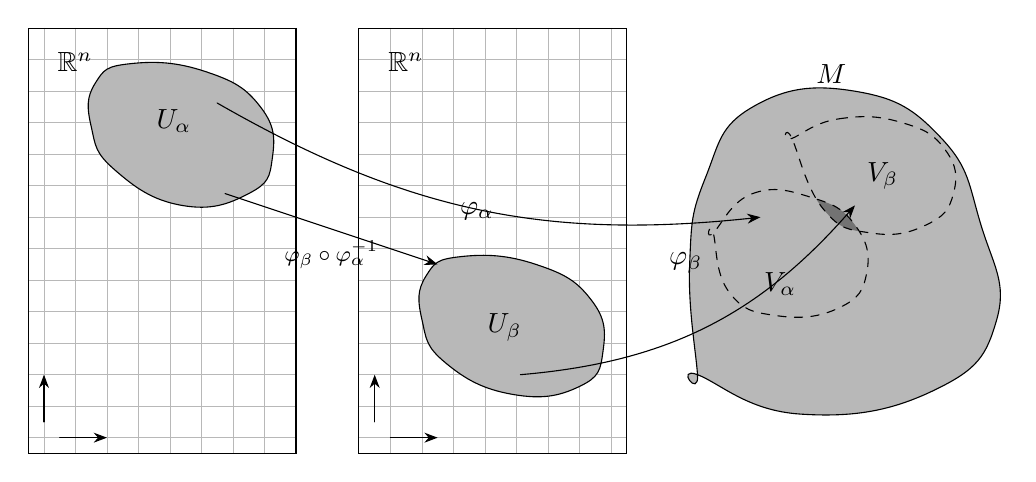
\begin{tikzpicture}[>=Stealth, line cap=round]
% ---------- 左一：R^n 与坐标域 U_alpha ----------
\draw[fillB, very thin] (0.2,0.2) grid[xstep=0.4,ystep=0.4] (3.6,5.6);
\draw (0.2,0.2) rectangle (3.6,5.6);
\draw[->] (0.6,0.4) -- (1.2,0.4);
\draw[->] (0.4,0.6) -- (0.4,1.2);
\node[anchor=north west] at (0.45,5.42) {$\mathbb R^n$};
\fill[fillB] plot[smooth cycle, tension=0.8] coordinates {(1.05,4.9) (1.5,5.15) (2.45,5.05) (3.15,4.6) (3.3,3.95) (3.0,3.5) (2.15,3.35) (1.3,3.8) (1.0,4.35)};
\draw plot[smooth cycle, tension=0.8] coordinates {(1.05,4.9) (1.5,5.15) (2.45,5.05) (3.15,4.6) (3.3,3.95) (3.0,3.5) (2.15,3.35) (1.3,3.8) (1.0,4.35)};
\node at (2.05,4.42) {$U_\alpha$};
% ---------- 左二：R^n 与坐标域 U_beta ----------
\draw[fillB, very thin] (4.4,0.2) grid[xstep=0.4,ystep=0.4] (7.8,5.6);
\draw (4.4,0.2) rectangle (7.8,5.6);
\draw[->] (4.8,0.4) -- (5.4,0.4);
\draw[->] (4.6,0.6) -- (4.6,1.2);
\node[anchor=north west] at (4.65,5.42) {$\mathbb R^n$};
\fill[fillB] plot[smooth cycle, tension=0.8] coordinates {(5.25,2.45) (5.7,2.7) (6.65,2.6) (7.35,2.15) (7.5,1.5) (7.2,1.05) (6.35,0.95) (5.5,1.35) (5.2,1.9)};
\draw plot[smooth cycle, tension=0.8] coordinates {(5.25,2.45) (5.7,2.7) (6.65,2.6) (7.35,2.15) (7.5,1.5) (7.2,1.05) (6.35,0.95) (5.5,1.35) (5.2,1.9)};
\node at (6.25,1.8) {$U_\beta$};
% 转移映射
\draw[->] (2.7,3.5) -- (5.4,2.6);
\node at (4.05,2.72) {\footnotesize $\varphi_\beta\circ\varphi_\alpha^{-1}$};
% ---------- 右：流形 M 与像集 ----------
\fill[fillB] plot[smooth cycle, tension=0.8] coordinates {(8.7,1.2) (10.0,0.7) (11.7,1.0) (12.5,1.9) (12.3,3.1) (11.8,4.2) (10.7,4.8) (9.4,4.6) (8.8,3.7) (8.6,2.6) (8.7,1.2)};
\draw plot[smooth cycle, tension=0.8] coordinates {(8.7,1.2) (10.0,0.7) (11.7,1.0) (12.5,1.9) (12.3,3.1) (11.8,4.2) (10.7,4.8) (9.4,4.6) (8.8,3.7) (8.6,2.6) (8.7,1.2)};
\begin{scope}
  \clip plot[smooth cycle, tension=0.8] coordinates {(8.9,3.0) (9.4,3.5) (10.15,3.45) (10.7,3.1) (10.85,2.5) (10.5,2.05) (9.7,1.95) (9.1,2.25) (8.9,3.0)};
  \fill[fillA] plot[smooth cycle, tension=0.8] coordinates {(9.9,4.2) (10.5,4.45) (11.3,4.4) (11.85,4.05) (11.95,3.5) (11.6,3.1) (10.9,3.0) (10.3,3.3) (9.9,4.2)};
\end{scope}
\draw[dashed] plot[smooth cycle, tension=0.8] coordinates {(8.9,3.0) (9.4,3.5) (10.15,3.45) (10.7,3.1) (10.85,2.5) (10.5,2.05) (9.7,1.95) (9.1,2.25) (8.9,3.0)};
\draw[dashed] plot[smooth cycle, tension=0.8] coordinates {(9.9,4.2) (10.5,4.45) (11.3,4.4) (11.85,4.05) (11.95,3.5) (11.6,3.1) (10.9,3.0) (10.3,3.3) (9.9,4.2)};
\node at (9.75,2.35) {$V_\alpha$};
\node at (11.05,3.72) {$V_\beta$};
\node at (10.4,5.02) {$M$};
% 坐标映射
\draw[->] (2.6,4.65) to[bend right=18] (9.5,3.2);
\node at (5.9,3.28) {$\varphi_\alpha$};
\draw[->] (6.45,1.2) to[bend right=22] (10.7,3.35);
\node at (8.55,2.62) {$\varphi_\beta$};
\end{tikzpicture}
\end{document}
